Membrane energy is a well-used function in mesh optimization~\cite{Kobbelt:1998} and can be minimized using the discrete Laplacian operator.  Here we use Laplacian smoothing due to its simplicity and good performance~\cite{Kobbelt:1998,Ohtake2001789,Chen2005376}, although we modify it to accommodate image-based edge information.  In addition, rather than apply Laplacian smoothing after the fact, entailing an iterative optimization~\cite{Kobbelt:1998}, we show that Laplacian smoothing can be incorporated directly into the least squares mesh estimation.  This has a number of  advantages.  First the smoothing penalty is traded off against measurement error rather than vertex offset.  Second, the due to our ray constraints on the vertices we are able to derive a linear least squares solution to the Laplacian avoiding the need to iterate as in methods such as~\cite{Kobbelt:1998}.  Finally  when the regularization components are added to Eq.~(\ref{eq:meshleastsquares}) they ensure that the solution is well-posed even when some of the facets have no depth points in them.

Laplacian smoothing uses an umbrella-operator~\cite{Kobbelt:1998} on a vertex, $\vertex$, and its neighbors $\vertex_i\in\mathcal{N}(\vertex)$,
\beq
\vect{u}(\vertex) = \frac{1}{n}\sum_{\vertex_i\in\mathcal{N}} \vertex_i - \vertex,\label{eq:umbrella}
\eeq
for $n$ neighbors as illustrated in Figure~\ref{fig:laplacian}.  In our model the vertices lie along known rays and so this operator can be expressed as a function of the vertex depth: $\vect{u}(\lambda) = \frac{1}{n}\sum_{i\in\mathcal{N}} \lambda_i \hvertex_i - \lambda\hvertex$.  The squared magnitude $\|\vect{u}(\lambda)\|^2$ is a natural penalty term as it captures a discrete form of the membrane energy.  Summing this over all vertices and arranging the known $\hvertex$ components into a single matrix $U$, we obtain
\beq
E_{reg}(\vlambda_v) = \| U \vlambda \|^2. \label{eq:reg}
\eeq

\begin{figure}
\begin{center}
   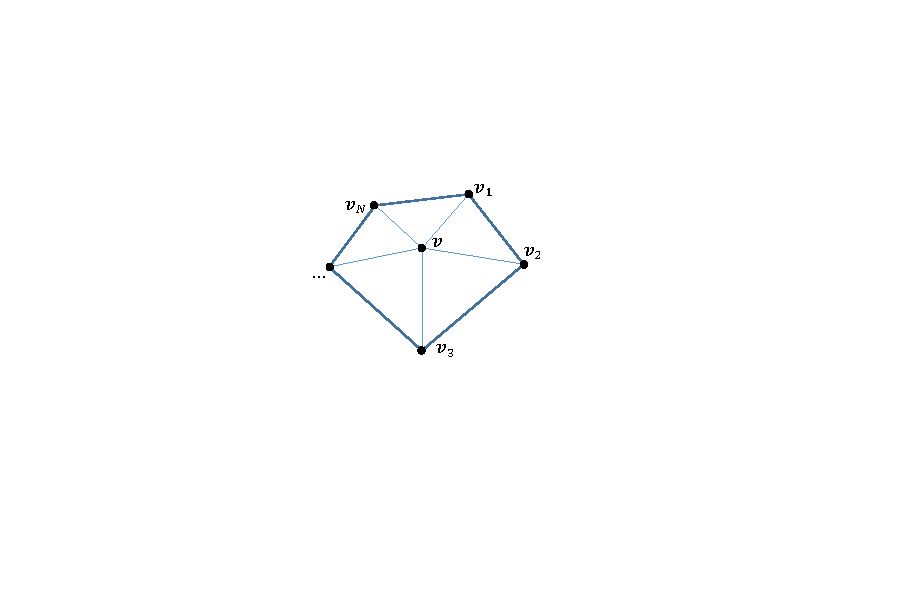
\includegraphics[trim=100 110 140 90,clip,width=0.8\linewidth]{Figures/LaplacianFacets}
\end{center}
   \caption{In discrete form the Laplacing is implemented as an umbrella operator, Eq.~(\ref{eq:umbrella}), over a vertex $\vertex$ and its first neighbors.}
\label{fig:laplacian}
\end{figure}

The cost in Eq. (\ref{eq:reg}) penalizes high curvature regions, and so provides a way incorporate smoothness priors into the mesh estimation.  Now we may have image cues for creases or sharp edges on portions of a mesh, as we describe in section \ref{sec:colormesh}.  We can modify the umbrella operator from Eq. (\ref{eq:umbrella}) so that the neighbors are only other vertices on the crease.  In this way the Laplacian acts along the crease, and not across it, allowing sharper folding along these edges.
 
 
 